% !TEX encoding = UTF-8 Unicode 
\section{Ausgewählte Problemstellungen}
%%%%%%
\subsection{Die Effektverkettung}
\paragraph{Das Modell}
VSTForx soll Plugins laden und mittels ''virtueller'' Kabel verbinden können. Als mathematisches Modell ist für diese Aufgabe der gerichtete Graph geeignet. Die Knoten repräsentieren die Plugins und die Kanten die Verbindungen.
\paragraph{Die Berechnungsreihenfolge}
Wie bereits in Kapitel \ref{Prozess} beschrieben erzeugt ein Plugin seine Ausgabe anhand einer ''processReplace'' Methode. Das Programm muss nun den beschriebenen Prozessablauf mit den geladenen Plugins durchführen. Doch in welcher Reihenfolge sollten diese Aufrufe stattfinden?\\\\
\begin{figure}[h]
	\centering
 	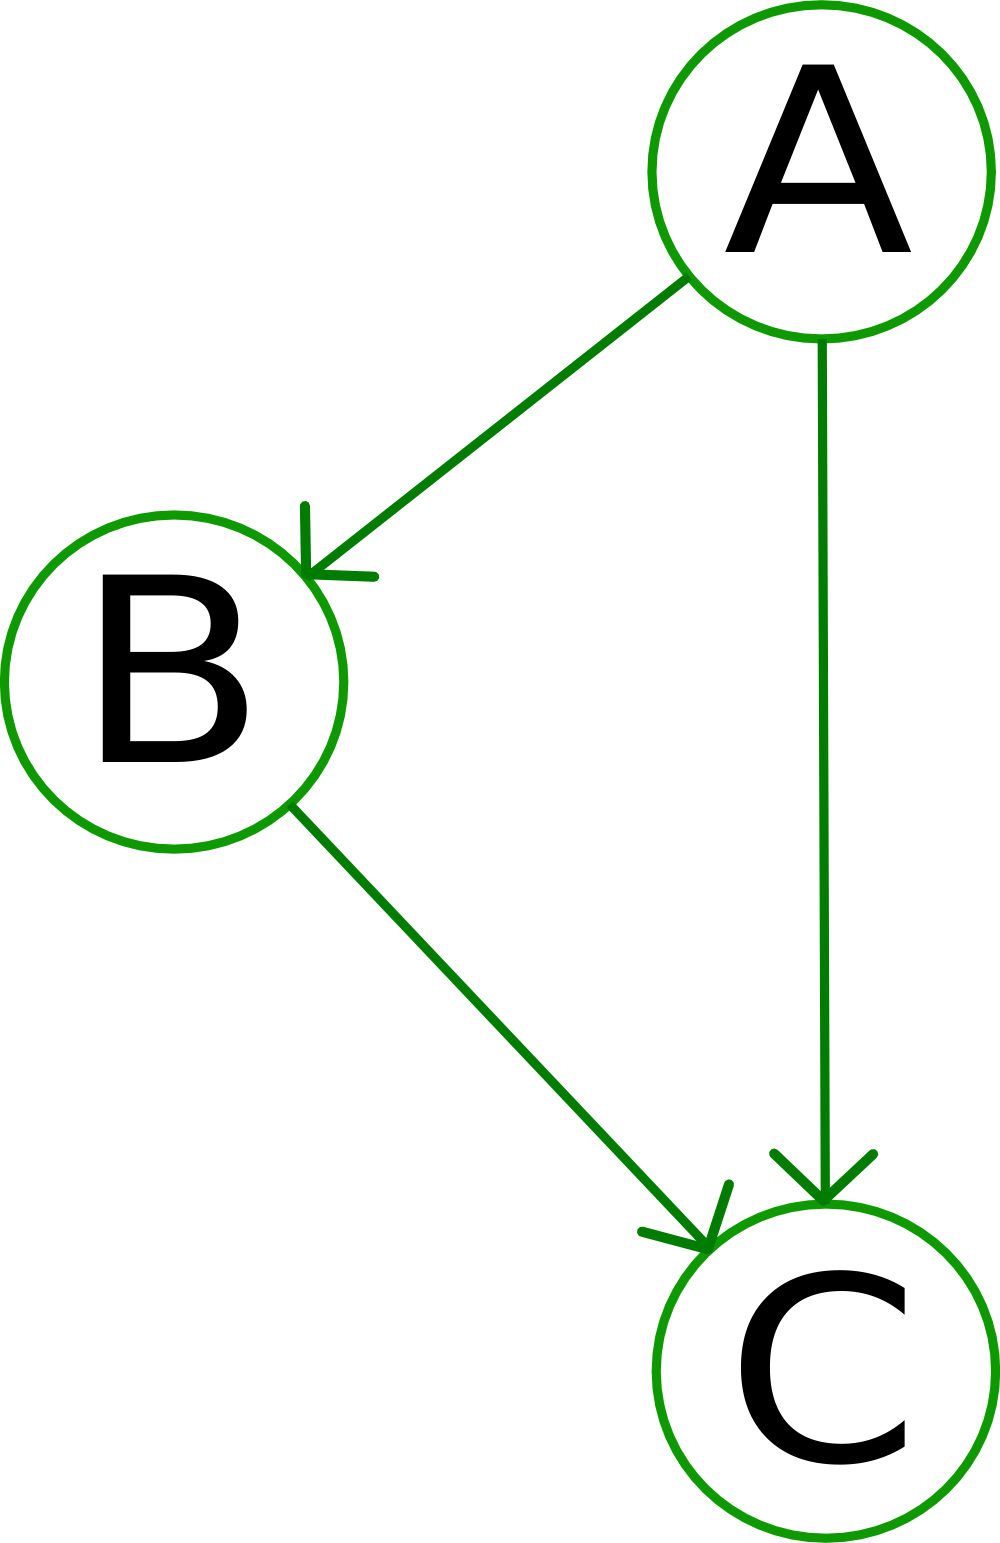
\includegraphics[scale=0.1]{../graphics/g01.png}
	\caption{Beispiel eines Plugin Graphen}
	\label{g01}
\end{figure}
Gegeben sei folgendes Beispiel:
\\\\
Jeder Knoten entspricht einem Plugin (A-C). Eine gerichtete Kante entspricht einer Verbindung von Pluginausgang zu Plugineingang.
\\\\
Der erforderliche Prozessablauf für Abbildung \ref{g01} wäre:
\begin{enumerate}
	\item bereite Inputsampleblöcke für Plugin-A vor
	\item führe ''processReplace'' mit Plugin-A aus
	\item bereite Inputsampleblöcke für Plugin-B vor (mit der Ausgabe von Plugin-A)
	\item führe ''processReplace'' mit Plugin-B aus
	\item\label{PlugC}bereite Inputsampleblöcke für Plugin-C vor (mit der Ausgabe von Plugin-A und B)
	\item führe ''processReplace'' mit Plugin-C aus
	\item übertrage die Ausgabe von Plugin-C in die Programm(VSTForx) Ausgabesampleblöcke
\end{enumerate}
Wie in Schritt \ref{PlugC} zu sehen ist zur korrekten Ausführung von Plugin-C notwendig, dass die Plugins A und C bereits bearbeitet wurden. Das bedeutet: Plugin-C ist von Plugin-A und Plugin-B abhängig. \\\\
In der Graphentheorie gibt es einen Algorithmus der in der Lage ist Abhängigkeiten aufzulösen: Die Topologische Sortierung.
\\\\
Die Topologische Sortierung basiert auf der Durchlaufstrategie Tiefensuche\footnote{oder auch DFS - engl.: Depth First Search}. \\
''Sie erzeugt eine lineare Anordnung von Knoten eines Graphen. Existiert eine Kante zwischen den Knoten (u, v),  so wird u vor v geordnet."\cite{bgl01}\\
Das Resultat der Topologischen Sortierung ist daher eine sortierte Menge an Knoten deren Reihenfolge  genau ihren Abhängigkeiten entspricht.
In unsrem Beispiel würde die Topologische Sortierung die (Plugin-)Knotenmenge \{A, B, C\}\footnote{vorausgesetzt Knoten A ist der Startknoten der Topologischen Sortierung} ergeben.
\paragraph{Rückkopplungen}
Eine Einschränkung der Topologischen Sortierung ist es, dass die zu sortierenden Graphen keine Zykel enthalten dürfen. Dies hat für VSTForx zur Auswirkung dass keine Rückkopplungen ''geschaltet'' werden können. Eine Rückkopplung wäre es zum Beispiel, wenn der Ausgang eines Plugins, direkt oder über Umwege, wieder an seinem Eingang liegen würde. Sollten Rückkopplungsschaltungen unterstützt werden, könnte man die betreffenden Knoten lokalisieren und in einen Subgraphen substituieren. Dieser Subgraph könnte dann die Knoten durch einen alternativen Algorithmus, einen der Rückkopplungen unterstützt, behandeln. Dies ist jedoch nicht vorgesehen. \\
Die Topologischen Sortierung ist es allerdings in der Lage zu erkennen ob ein Graph Zyklisch ist. Zur Vermeidung von Fehlverhalten werden daher Zyklische Graphen nicht zugelassen.  
\paragraph{Inaktive Knoten}
%%%%%%
\subsection{Das Latenzproblem}
%%%%%%
\subsection{Persistenz}
%%%%%%
\subsection{Portabilität}
%%%%%%
\subsection{Nebenläufigkeit}
%%%%%%
\subsection{Verwendung von Speicherdateien auf unterschiedlichen Systemen}